% Copyright 2023 Riley Hanus, PhD
% Unauthorized copying and use of this file, via any medium is strictly prohibited
% Proprietary and confidential
% Written by Riley Hanus <hanusriley@gmail.com>, November 2023

\documentclass{article}
% Copyright 2022 Riley Hanus, PhD
% Unauthorized copying and use of this file, via any medium is strictly prohibited
% Proprietary and confidential
% Written by Riley Hanus <hanusriley@gmail.com>, November 2022

\usepackage[framemethod=TikZ]{mdframed} 
\usepackage{verbatim}
\usepackage{hyperref}
\usepackage{xstring}
\usepackage{listofitems}
\usepackage{substr}
\usepackage{cprotect}

%%%%%%%%%%%%%%%%%%%%%%%%%%%%%%%%%%%%%%%%%%%%%%%%%%%%%%%%%%%%%%
% iframe environment for embedding <iframe ...></iframe>     %
% result: html=embedded iframe, pdf=multimedia box w/ href   %
%%%%%%%%%%%%%%%%%%%%%%%%%%%%%%%%%%%%%%%%%%%%%%%%%%%%%%%%%%%%%%

\newenvironment{iframe}[1][]{%
\ifstrempty{#1}%
{\mdfsetup{%
frametitle={%
\tikz[baseline=(current bounding box.east),outer sep=0pt]
\node[anchor=east,rectangle,fill=blue!20]
{\strut Digital Content};}}
}%
{\mdfsetup{%
frametitle={%
\tikz[baseline=(current bounding box.east),outer sep=0pt]
\node[anchor=east,rectangle,fill=blue!20]
{\strut Digital Content~:~#1};}}%
}%
\mdfsetup{innertopmargin=10pt,linecolor=blue!20,%
linewidth=2pt,topline=true,%
frametitleaboveskip=\dimexpr-\ht\strutbox\relax
}
\begin{mdframed}[]}{\end{mdframed}}

\newcommand{\parseiframe}[1]{\setsepchar{"}\readlist\iframelist{#1}
}

\newcommand{\iframeurl}[2]{
    \parseiframe{#1}
    \foreachitem \i \in \iframelist{
        \IfSubStringInString{://www.}{\i}{ \let\result=\i}{}
    }
    \href{\result}{#2}
}

\newcommand{\InsertIframe}[4]{
    % #1: html code for <iframe>
    % #2: display name for hyperlink in 'Digital Content box' in pdf
    % #3: caption
    % #4: type of media for 'Digital Content: xxx'
   \begin{iframe}[#4]
      \iframeurl{#1}{#2} | #3
   \end{iframe}
}

%%%%%%%%%%%%%%%%%%%%%%%%%%%%%%%%%%%%%%%%%%%%%%%%%%%%%%%%%%%%%%%
% html environment for inserting custom html <div ...></div>  %
% result: html=html code, pdf=latex code                      %
%%%%%%%%%%%%%%%%%%%%%%%%%%%%%%%%%%%%%%%%%%%%%%%%%%%%%%%%%%%%%%%

\newenvironment{customhtml}{}{}

\newcommand{\InsertHTML}[2]{
    % #1: html code for compiled html
    % #2: latex code for compiled pdf 
   \begin{customhtml}
      #2
   \end{customhtml}
}

%%%%%%%%%%%%%%%%%%%%%%%%%%%%%%%%%%%%%%%%%%%%%%%%%%%%%%%%%%%%%%%%%%%%%%%%%%%%%%%%
% calchub environment: for embedding a calchub workspace                       %
% texedbook compatible: html=embedded work space, pdf=multimedia box w/ href   %
%%%%%%%%%%%%%%%%%%%%%%%%%%%%%%%%%%%%%%%%%%%%%%%%%%%%%%%%%%%%%%%%%%%%%%%%%%%%%%%%
\newenvironment{calchub}
    {\begin{iframe}[CalcHub Workspace]
    }
    {\end{iframe}
    }

\newcommand{\InsertCalchub}[3]{ 
   % 1st input: href 
   % 2nd input: display name
   % 3rd input: description
   \begin{calchub}
      \href{#1}{#2} | #3
   \end{calchub}
} 


%%%%%%%%%%%%%%%%%%%%%%%%%%%%%%%%%%%%%%%%%%%%%%%%%%%%%%%%%%%%%%%%%%%%%%%%%%%%%%%%
% video environment: for embedding videos                                      %
% texedbook compatible: html=embedded video, pdf=multimedia box w/ href        %
%%%%%%%%%%%%%%%%%%%%%%%%%%%%%%%%%%%%%%%%%%%%%%%%%%%%%%%%%%%%%%%%%%%%%%%%%%%%%%%%
\newenvironment{youtube}
   {\begin{iframe}[Video]
   }
   {\end{iframe}
   }

\newcommand{\InsertYouTube}[3]{ 
   % 1st input: href   
   % 2nd input: display name 
   % 3rd input: description
   \begin{youtube}
      \href{#1}{#2} | #3
   \end{youtube}
} 

%%%%%%%%%%%%%%%%%%%%%%%%%%%%%%%%%%%%%%%%%%%%%%%%%%%%%%%%%%%%%%%%%%%%%%%%%%%%%%%%
% python coding environment: for coding practice                               %
% texedbook compatible: html=embedded trinket, pdf=multimedia box w/ href      %
%%%%%%%%%%%%%%%%%%%%%%%%%%%%%%%%%%%%%%%%%%%%%%%%%%%%%%%%%%%%%%%%%%%%%%%%%%%%%%%%


\newenvironment{trinket}
   {\begin{iframe}[Python coding environment]
   }
   {\end{iframe}
   }

\newcommand{\InsertTrinket}[3]{ 
   % 1st input: href   
   % 2nd input: display name 
   % 3rd input: description
   \begin{trinket}
      \href{#1}{#2} | {#3}
   \end{trinket}
} 


%%%%%%%%%%%%%%%%%%%%%%%%%%%%%%%%%%%%%%%%%%%%%%%%%%%%%%%%%%%%%%%%%%%%%%%%%%%%%%%%
% panopto environment: for viewing videos hosted by panopto                    %
% texedbook compatible: html=embedded iframe, pdf=multimedia box w/ href       %
%%%%%%%%%%%%%%%%%%%%%%%%%%%%%%%%%%%%%%%%%%%%%%%%%%%%%%%%%%%%%%%%%%%%%%%%%%%%%%%%


\newenvironment{panopto}
   {\begin{iframe}[Video]
   }
   {\end{iframe}
   }

\newcommand{\InsertPanoptoVideo}[3]{ 
   % 1st input: href   
   % 2nd input: display name 
   % 3rd input: description
   \begin{panopto}
      \href{#1}{#2} | {#3}
   \end{panopto}
} 

% Mathjax equation referencing
\newcommand\mjref[1]{\ref{#1}}



\title{Author's guide to texedbook}
\author{Riley Hanus, PhD}
\date{}

\begin{document}
 
\maketitle

\begin{abstract}
The \verb'texedbook' code base is a tool for publishing articles, educational content, and textbooks online without the need to learn html, css, and javascript. The author writes the content following this guide, compiles it using \verb'latexmk', and after following the set-up instructions in the \verb'README.md' runs 
\begin{verbatim}
python make_texedbook.py ./path/to/latex/project/directory
\end{verbatim}
which generates a collection of html and css files in \verb'./output/' that can be directly published online. The product is a computer and mobile friendly webpage, with all document features preserved and all content embedded.  In addition to supporting most of the native latex features, \verb'texedbook' provides tools for embedding digital and interactive content such as videos, quizzes, code editors and compilers, etc. 

This article acts as an author's guide to \verb'texedbook' (\verb'tex': Latex based, \verb'ed': education focused, \verb'book': classic textbook functionality maintained) and will demonstrate the document features that are explicitly supported, and the specific way they must be used to ensure a clean output html page.  First, the native latex capabilities will be demonstrated including figures, equations, tables, cross-referencing, citations, etc. Then the \verb'texedbook' specific features will be presented which allow the author to embed digital content (anything that can be contained in an iframe) into the resulting webpage straight from the latex document. 
\end{abstract}

\section{Motivation for texedbook project}

When writing anything technical in nature, the need for proper writing tools is glaring. Without a framework to efficiently manage citations, cross-reference document items (e.g. sections, equations, figures), write math, etc., writing anything with technical substance becomes prohibitively difficult. Latex, despite its quirks, is a very good framework to manage these critical writing tools and compiling beautifully typeset pdf documents.

At the same time, publishing and education has transitioned to a digital-first experience for the consumer, yet publishers still cling to a print-first model. There is a clear need for a tool enabling authors to publish digital-first articles, books, and courses. The natural medium for this digital-first publishing is an html, css, and javascript based webpage. 

\verb'texedbook' combines the strengths of latex for authoring articles and books with the versatility and universality of an interactive webpage.  

\section{Required file naming and structure}
\verb'texedbook' requires specific file naming and those files must live in specific locations within your project directory. This ensures proper handling of figures and that the html code generated from your project can be templated properly into your final result. 

Specifically, the main latex document must be called \verb'main.tex' and must be in the base of your project directory. \verb'texedbook_envs.tex' contains required commands and environments, and best practice is to leave it right next to \verb'main.tex'. In addition, if your project has references, it is best practice to leave \verb'references.bib' next to \verb'main.tex' as well. You may use \verb'\input{doc1}' in the preamble and \verb'\include{doc2}' in the document as usual. However, they must be called as \verb'\include{doc2}', not \verb'\include{doc2.tex}' since will tell the \verb'latexpand' command (native to the full latex installation and used here) to look for \verb'doc2.tex.tex'.  Any figures your project may have must be in pdf format and must live in a \verb'figures/' directory which itself lives next to \verb'main.tex'.  

\begin{verbatim}
    main-project-directory/
        main.tex (required)
        texedbook_envs.tex (required)
        doc1.tex
        doc2.tex
        references.bib
        figures/ (required)
            figure-1.pdf
\end{verbatim}


\section{Native latex features} \label{sec:latexfeatures}
This section will provide a non-exhaustive documentation of the native latex features that are supported by \verb'texedbook'. It will also provide their specific usage that yields a clean html output.

\subsection{Figures}
All figures used in the document must be contained in a directory named \verb'./figures/' and that folder must be located in the same location as \verb'main.tex'. In addition, all figures must be in pdf format.

Ensuring that figures are displayed correctly in the resulting html is tricky. The simplest and most effective way is to assign that \textbf{all figures span width of the text on the page}. This display condition reliably converts from latex to html and translates from computer to mobile formats well, which is not the case for all display options. Since the aspect ratio of figures is locked by design, this may cause your figure to display very large in the pdf and html. If you would like the figure to display smaller, simply add white space to the left and right of the pdf as is done in Figure \ref{fig:example}.

An example of the latex code used to add a figure is below.
\begin{verbatim}
    \begin{figure}[t]
        \centering
        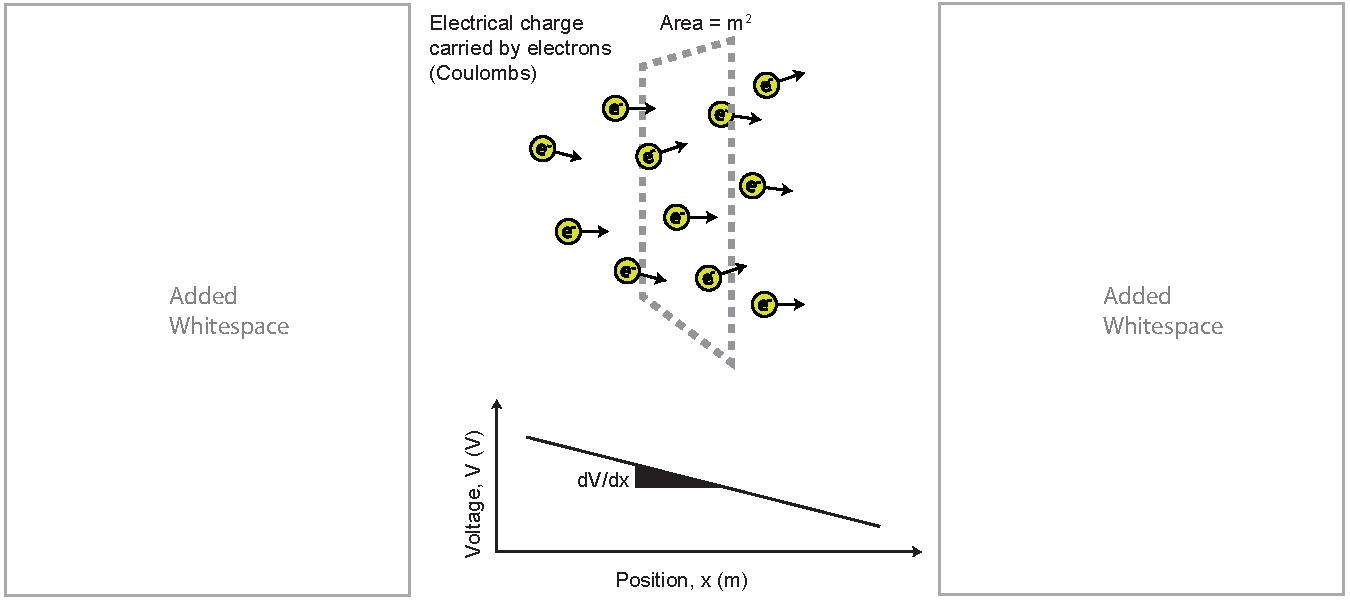
\includegraphics[width=0.99\textwidth, keepaspectratio]{figures/fig.pdf}
        \caption{Example figure.}
        \label{fig:example}
    \end{figure}  
\end{verbatim}
The \verb'[t]' places the figure at the top of a page in the pdf, and does nothing to the html output. The html output will place the figure where it appears in the code. The \verb'\centering' center justifies the figure. The \verb'\includegraphics[]{}' adds in the figure, the \verb'width=0.99\textwidth' sets the width of the figure to 99\% of the text width, and the \verb'figures/fig.pdf' points to the figure which must be placed in a \verb'./figures/' directory and must be pdf format. The \verb'\label' allows the figure to be cross-referenced. 

\begin{figure}[t]
    \centering
    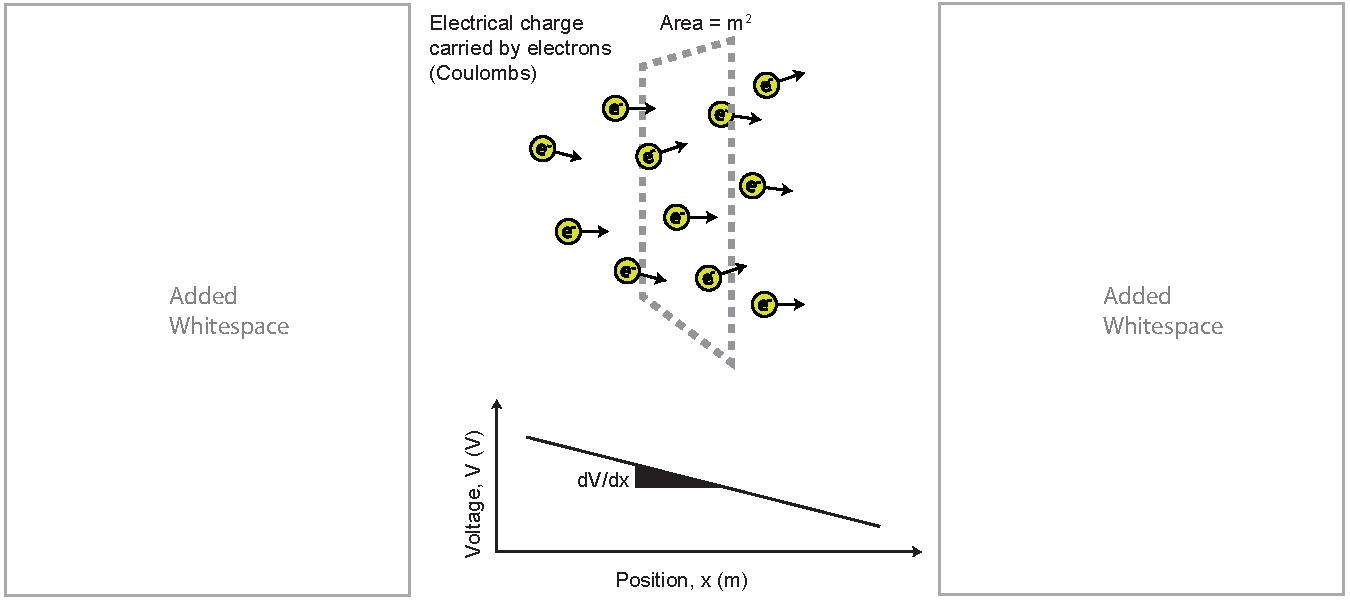
\includegraphics[width=0.99\textwidth, keepaspectratio]{figures/fig.pdf}
    \caption{Example figure. Since the convention for texedbook is for figures to span the text width, whitespace is added to control size of the image.}
    \label{fig:example}
\end{figure}

\subsection{Equations} \label{sec:equations}
Equations are an inherently tricky problem for digital publishing. The core of the problem lies in the fact that html was designed around the standard alphanumeric alphabet, and math requires a wider range of complex symbols and typesetting. The default usage of \verb'texedbook' leverages \verb'mathjax', allowing all the native latex equations to be reliably reproduced in the html output.

In line equations can be included $n\lambda=2d \sin \theta$, as well as displayed equations 
\begin{equation}
    n\lambda=2d \sin \theta.
    \label{eq:braggslaw}
\end{equation}
Cross-referencing equations is done using the \verb'\mjref' function provided in \verb'texedbook_envs.tex'. For example, Eq. \mjref{eq:braggslaw} is Bragg's Law which is commonly used to find diffraction conditions of light of wavelength $\lambda$ interacting with a crystal with lattice spacing $d$ at an incident angle of $\theta$. The \verb'\mjref' function simply substitutes \verb'\ref' when the latex is compiled. However, when \verb'tex4ebook' converts the project to html, the \verb'aux/config.cfg' file tells \verb'tex4ebook' to insert \verb'\eqref' in place of all \verb'\mjref's, which \verb'mathjax' knows to look for in the html and use for equation numbering and cross-referencing. 

\subsection{Tables}
Tables are inherently difficult to write in latex. \href{https://www.tablesgenerator.com/}{Tables Generator} is a great tool for generating latex code for tables. Note that the table styling in the html output is different then the latex output. 

An example of the latex syntax for including a table is given below.
\begin{verbatim}
    \begin{table}[t]
        \caption{Example table.}
        \centering
        \begin{tabular}{|c|c|...}
        ...
        \end{tabular}
        \label{table:example}
    \end{table}
\end{verbatim}

The \verb'[t]' places the table at the top of a page in the pdf, and does nothing to the html output. The html output will place the table where it appears in the code. The \verb'\centering' center justifies the table. The table syntax goes within \verb'\tabular' environment. The \verb'\label' allows the table to be cross-referenced. 

\begin{table}[t]
    \caption{Example table.}
    \centering
    \begin{tabular}{|c|c|c|c|}
    \hline
    \multicolumn{1}{|l|}{Sample} & \multicolumn{1}{l|}{Data 1} & \multicolumn{1}{l|}{Data  2} & \multicolumn{1}{l|}{Data 3} \\ \hline
    A                            & 53                          & 62                           & 75                          \\ \hline
    B                            & 51                          & 61                           & 72                          \\ \hline
    C                            & 58                          & 69                           & 71                          \\ \hline
    \end{tabular}
    \label{table:example}
\end{table}

\subsection{Code Syntax}
Code syntax can be displayed using the verbatim environment native to latex 
\begin{verbatim}
\begin{verbatim}
    for i in list:
        print('some code')
\end{verbatim } 
\end{verbatim}
This will render in the html as a displayed code block that scrolls if a text overflow happens. This way readers will never miss the syntax they need, no matter the size of thier screen.

Code can be written in-line using the \verb'\verb' function. This function comes from the \verb'verbatim' package and is unique in that it doesn't use the curly brackets for its argument. As implemented here, it cannot be used as an argurment in most commands such as, \verb'\section{}' or \verb'\caption{}'. It takes the first non-letter character as the open argument and looks for that same character again to close the argument. I typically use \verb_\verb'code here'_. This is meant for short (one word) expressions; if the content is too long it will be cut off. For long syntax use the \verb'\begin{verbatim}' environment.    

\subsection{Cross-referencing and hyperlinks}
Cross-referencing can be used as normal in latex and all the hyperlinking functionality will be preserved in the html. For example, Section \ref{sec:latexfeatures}, Table \ref{table:example}, and Figure \ref{fig:example}. The only important exception is Equations where the \verb'\mjref' command must be used such that mathjax can properly label and cross-reference equations locally in the html page using javascript (see Section \ref{sec:equations}).

Hyperlinks to external webpages can be added in latex using the \verb'\href' command.
\begin{verbatim}
    \href{https://www.webpage.com}{Display name in document}
\end{verbatim}

\subsection{Citations}
The native bibliography features are maintained. For example, one can cite an article \cite{Hanus2021} or multiple articles \cite{Hanus2019,Hanus2021,Gregory2021}. Note that the hyperlinking to the bibliography in the pdf, a result of using the \verb'hyperref' package, is maintained in the resulting html. The default bibliography style used in \verb'texedbook' is \verb'unsrturl'. Note that this style supports hyperlinking to the url, and/or doi if that field is present in the .bib entry, and the hyperlinking is maintained in the resulting html. It is recommended that the doi field is used instead of the url, since line breaking needed to typeset urls is handled poorly by latex. Latex's performance on typesetting doi hyperlinks seems to work more reliably.

\section{Texedbook features}
This section will demonstrate special \verb'texedbook' environments and commands that allow the author to embed digital content directly from the latex code into the resulting webpage. There are several commands provided in \verb'texedbook_envs.tex' to achieve this. \verb'\InsertIframe' is specifically for iframes (explained in Section \ref{sec:iframes}) and \verb'\InsertHTML' is more generic and allows the author to include any html element they wish. The arguements the author inputs tells \verb'texedbook' what to render in the pdf as well as what to template into the output html. 

In practice, \verb'texedbook' searches the latex project for the specific pattern \verb'\InsertXXX{...}' and grabs the arguements needed to template the html into the final webpage. Therefore, the command and first arguement (e.g.) \verb'\InsertXXX{...}' must be occupy one line in the latex code. In addition, you will see an extra space before the open curly bracket when displaying the latex code syntax for these functions in this document. This avoids unintentionally triggering the templating functions in \verb'make_texedbook.py', and insures that this Author's Guide works properly. The author should also \textbf{avoid unintentionally triggering the templating functions by writing the exact synax for these commands in places it doesn't belong (e.g. in comments, verbatim enviroments, etc.).}

\subsection{Iframes} \label{sec:iframes}
An inline frame, or iframe, is an html element that loads a webpage within another webpage. For example, when you see a YouTube video on a website other than www.youtube.com, it is likely being placed their using an iframe. However, as you can infer from the definition, iframes are extremely versatile and can be used for far more than embedding YouTube videos. Essentially, anything online can be embedded using an iframe. Often times there will be a \textit{share} button next to a sharable feature on a webpage, and one of the sharing options is Often \textit{embed}, or have the \verb'<>' symbol. This option will provide a piece of html code for the iframe that looks something like this, which can be copy and pasted. 

\begin{verbatim}
    <iframe width="560" height="315" 
            src="https://www.youtube.com/embed/..." 
            title="YouTube video player" ...></iframe>
\end{verbatim}

Importantly, if there are any \verb'%' symbols in the html code, which is very common, you will need to add a backslash to `escape' the character. In this way your latex code should have \verb'\%' in place of all \verb'%'. This will avoid the \verb'%' symbol in the html from inadvertantly commenting out a portion of your command. \verb'texedbook' will fix the html code when templating.  

The \verb'\InsertIframe' command provided in \verb'texedbook_envs.tex' allows the author to embed any iframe into the output html, directly from the latex project. The pdf will display a \textit{digital content box} containing a hyperlink to the source URL contained in the iframe code. The output html will contain the iframe properly embedded. There are four arguments for \verb'\InsertIframe', and they are detailed here.
\begin{verbatim}
    \InsertIframe {<iframe ...></iframe> ('%'s replaced with '\%')}
                  {hyperlink display text}
                  {caption}
                  {type of digital content}
\end{verbatim}  

Below is this command in practice various free tools are embedded. As you can see in the compiled pdf, a fancy \textit{Digital Content} box and hyperlink are rendered. In the html output, the iframe is properly embedded.

\subsubsection{YouTube}
To embed a YouTube video, go to the video you wish to embed. Click the \textit{Share} button, then \textit{Embed}, then \textit{Copy}. The iframe html code is now copied to your clipboard. Paste it into the first argument of the \verb'\InsertIframe' command, and fill in the rest of the arguements. Remember to replace all \verb'%' that may be in the html code with \verb'\%'.

\InsertIframe{<iframe width="560" height="315" src="https://www.youtube.com/embed/zqtx0gA5K2s?si=nLdAne1jF961EMxx" title="YouTube video player" frameborder="0" allow="accelerometer; autoplay; clipboard-write; encrypted-media; gyroscope; picture-in-picture; web-share" allowfullscreen></iframe>}
             {Intro to Copyright Law}
             {MIT OpenCourseWare 6.912, Lecture 1}
             {Video} 

\subsubsection{Python coding environment}
There now exists a wonderful tool for running python within a web browser called \href{https://jupyterlite.readthedocs.io/en/stable/#}{JupyterLite}. Historically, python needed to be run locally on your computer, or if the code was being edited and ran in a web browser then it was actually compiled on a server somewhere with a python installation, which adds cost. With JupyterLite, a python coding enviroment, which runs a read-eval-print loop (REPL) locally in your browser, can be simply added using the following iframe. Note, the \verb'%' is aready replaced with \verb'\%' such that this exact html code can be pasted into the first arguement of the \verb'\InsertIframe' command.
\begin{verbatim}
    <iframe src="https://jupyterlite.github.io/demo/repl/index.html?kernel=python&toolbar=1&theme=JupyterLab Dark" width="100\%" height="500px"></iframe>
\end{verbatim}
Here, is this python REPL iframe in practice, and an example prompt.

Generate two arrays containing 10 random numbers each and plot one along the x-axis and the other along the y-axis.
\begin{verbatim}
    import numpy as np
    import matplotlib.pyplot as plt
    
    x = np.random.rand(10)
    print(x)
    y = np.random.rand(10)
    print(y)
    plt.plot(x,y, 
             linewidth=0, 
             marker="o", 
             color="black")
    plt.show()
\end{verbatim}

\InsertIframe{<iframe src="https://jupyterlite.github.io/demo/repl/index.html?kernel=python&toolbar=1&theme=JupyterLab Dark" width="100\%" height="500px"></iframe>}
              {Python Coding Eviroment}
              {An embedded Jupyter Notebook running python using JupyterLite}
              {JupyterLite}


\subsubsection{Google Form Quiz}
Google as a suite of free web applications. Google Forms is a great tool for making and administering quizzes. See this concise video for creating a Google Form Quiz.

\InsertIframe{<iframe width="560" height="315" src="https://www.youtube.com/embed/Pdt8Vv7-3Xk?si=C36HazkC1eybzlfo" title="YouTube video player" frameborder="0" allow="accelerometer; autoplay; clipboard-write; encrypted-media; gyroscope; picture-in-picture; web-share" allowfullscreen></iframe>}{Google From Quiz Tutorial}{A video explaining how to create a quiz in Google Forms with a focus on use in the classroom.}{Video}

To embed this quiz into your project, click the \textit{Share} button, the the \verb'<>' icon, then copy the iframe code and paste it into the first arguement of the \verb'\InsertIframe' command. A similar process can be used to embed other Google web applications into your project.
\InsertIframe{<iframe src="https://docs.google.com/forms/d/e/1FAIpQLSdVIM1ADBswXlDN_zVleaTG5WZIaAvu9jbqHfdzjQj1-P5Qzg/viewform?embedded=true" width="640" height="965" frameborder="0" marginheight="0" marginwidth="0">Loading…</iframe>}
             {Example Quiz}
             {Test your understanding of texedbook}
             {Google Form}

\subsection{Special embed commands}
There also may be scenerios when the embed code is not provided. This is the case for videos hosted on the course management platform Panopto. In this case simply replacing the `Video' with `Embed' in the url and placing it in a generic <iframe> element embeds the video properly. Therefore, special commands are provided which generates the <iframe> for the author with the following syntax. See all the special commands provided in \verb'texedbook_envs.tex'. An example for a Panopto video is given here.
\begin{verbatim}
    \InsertPanoptoVideo {https://www.url-to-video.com/xxx}
                        {hyperlink display text}
                        {caption}
\end{verbatim}  

Below is this command in practice, where a lecture from Prof. G. Jeff Snyder's course on electronic and thermal transport at Northwestern University is embedded. As you can see in the compiled pdf, a fancy \textit{Digital Content} box and hyperlink are rendered. In the html output, the iframe is properly embedded.

\InsertPanoptoVideo{https://northwestern.hosted.panopto.com/Panopto/Pages/Viewer.aspx?id=405416aa-29b1-462a-b861-aa2b00497f15&start=0}{MSE 485 2-11}{Prof. G. Jeff Snyder's lecture on Complex Fermi Surfaces}

\subsection{Generic HTML}
The author may desire more flexibility. The \verb'\IncludeHTML' command is quite generic and versitile. Its first argument is simply the html element that will be templated directly into the output html code. Its second arguement is the latex code that will be compiled into the pdf.   
\begin{verbatim}
    \InsertHTML {html code for output (e.g. <div ...></div>)}
                {latex code for compiled pdf}
\end{verbatim}  

See this command implemented below where another YouTube video is embedded in the output html, and a simple hyperlink is compiled in the pdf. 
\InsertHTML{<iframe width="560" height="315" src="https://www.youtube.com/embed/spUNpyF58BY?si=wW31fiDuXUkdEAQn" title="YouTube video player" frameborder="0" allow="accelerometer; autoplay; clipboard-write; encrypted-media; gyroscope; picture-in-picture; web-share" allowfullscreen></iframe>}
           {\href{https://www.youtube.com/embed/spUNpyF58BY?si=wW31fiDuXUkdEAQn}{Three Blue One Brown video on the Fourier Transform.}}


\bibliographystyle{unsrturl}
\bibliography{sample}

\end{document}

